\documentclass[border=10pt]{standalone}
\usepackage{tikz}
\usetikzlibrary{calc}

\begin{document}
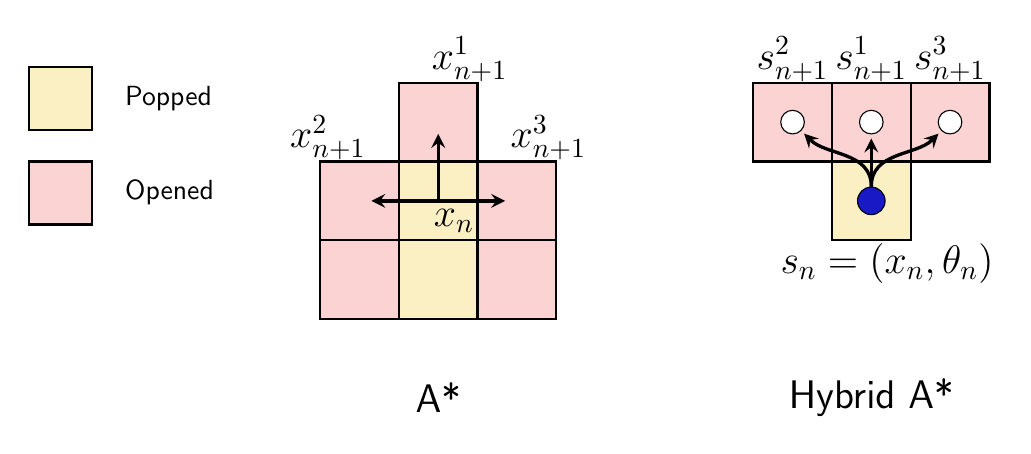
\begin{tikzpicture}[
    text=black,
    >={stealth},
    dot/.style={circle, fill=black!25!blue!90, draw=black, minimum size=3.5mm, inner sep=0pt},
    hollowcircle/.style={circle, draw=black, fill=white, minimum size=3mm, inner sep=0pt},
    arrowline/.style={->, shorten >=0.5mm, very thick},
    box/.style={draw=black, thick}
]

% Define custom colors to match the image closely
\definecolor{myyellow}{HTML}{FAF0C4}
\definecolor{mypink}{HTML}{FCD3D3}

% ==================== LEGEND ====================
\begin{scope}[shift={(-4, 0.5)}]
    % Popped Legend
    \draw[box, fill=myyellow] (-1.2, 0.4) rectangle (-0.4, 1.2);
    \node[anchor=west] at (-0.1, 0.8) {\textsf{Popped}};

    % Opened Legend
    \draw[box, fill=mypink] (-1.2, -0.8) rectangle (-0.4, 0);
    \node[anchor=west] at (-0.1, -0.4) {\textsf{Opened}};
\end{scope}

% ==================== A* DIAGRAM ====================
\begin{scope}[shift={(0, 0)}]
    % Grid Cells
    % Middle column (Yellow)
    \draw[box, fill=myyellow] (-0.5, -1.5) rectangle (0.5, -0.5);
    \draw[box, fill=myyellow] (-0.5, -0.5) rectangle (0.5, 0.5);
    
    % Left column (Pink)
    \draw[box, fill=mypink] (-1.5, -1.5) rectangle (-0.5, -0.5);
    \draw[box, fill=mypink] (-1.5, -0.5) rectangle (-0.5, 0.5);
    
    % Right column (Pink)
    \draw[box, fill=mypink] (0.5, -1.5) rectangle (1.5, -0.5);
    \draw[box, fill=mypink] (0.5, -0.5) rectangle (1.5, 0.5);
    
    % Top cell (Pink)
    \draw[box, fill=mypink] (-0.5, 0.5) rectangle (0.5, 1.5);

    % Arrows
    \draw[arrowline] (0, 0) -- (0, 0.9);
    \draw[arrowline] (0, 0) -- (-0.9, 0);
    \draw[arrowline] (0, 0) -- (0.9, 0);

    % Labels
    \node at (0.4, 1.8) {\Large $x_{n+1}^1$};
    \node at (-1.4, 0.8) {\Large $x_{n+1}^2$};
    \node at (1.4, 0.8) {\Large $x_{n+1}^3$};
    \node at (0.2, -0.25) {\Large $x_n$};

    % Title
    \node at (0, -2.5) {\Large \textsf{A*}};
\end{scope}

% ==================== HYBRID A* DIAGRAM ====================
\begin{scope}[shift={(5.5, 0)}]
    % Grid Cells
    % Center (Yellow)
    \draw[box, fill=myyellow] (-0.5, -0.5) rectangle (0.5, 0.5);
    
    % Top cells (Pink)
    \draw[box, fill=mypink] (-1.5, 0.5) rectangle (-0.5, 1.5);
    \draw[box, fill=mypink] (-0.5, 0.5) rectangle (0.5, 1.5);
    \draw[box, fill=mypink] (0.5, 0.5) rectangle (1.5, 1.5);

    % Nodes
    \node[dot] (start) at (0, 0) {};
    \node[hollowcircle] (h1) at (0, 1) {};
    \node[hollowcircle] (h2) at (-1, 1) {};
    \node[hollowcircle] (h3) at (1, 1) {};

    % Arced kinematic lines
    \draw[arrowline] (start) to[out=90, in=-45] (h2);
    \draw[arrowline] (start) to[out=90, in=-90] (h1);
    \draw[arrowline] (start) to[out=90, in=225] (h3);

    % Labels
    \node at (-1, 1.8) {\Large $s_{n+1}^2$};
    \node at (0, 1.8) {\Large $s_{n+1}^1$};
    \node at (1, 1.8) {\Large $s_{n+1}^3$};
    \node at (0.2, -0.8) {\Large $s_n = (x_n, \theta_n)$};

    % Title
    \node at (0, -2.5) {\Large \textsf{Hybrid A*}};
\end{scope}

\end{tikzpicture}
\end{document}